\chapter{Evaluating \Edgeworth{}}
\label{chp:edgeworth-eval}

\section{Overview and Research Questions}

To effectively scale up visual practice authoring, \Edgeworth must support a diverse set of instructional domains, generate high-quality diagrams consistently, and allow educators to author real-world problems. In \cref{sec:edgeworth-case-studies,sec:reliability-eval,sec:expert-feedback}, we evaluate \Edgeworth by answering the following research questions on these qualities:

\begin{enumerate}[label=RQ\arabic*]
    \item\label{rq:dom} \textbf{Expressiveness}: Can \Edgeworth generate meaningful diagram mutants in multiple domains of instruction?
    \item\label{rq:mut} \textbf{Reliability}: Can \Edgeworth reliably generate translation problems with relatively few variations required?
    \item\label{rq:eco} \textbf{Ecological validity}: Do real-world instructors consider \Edgeworth-generated translation problems to be useful? 
\end{enumerate}

First, to show the expressiveness of \Edgeworth, we performed case studies by recasting 31 problems from Euclidean geometry, discrete math, and general chemistry textbooks and courses (\cref{sec:case-studies}). Second, we evaluated the reliability of \Edgeworth by labeling 310 diagram variations from the recasted problems by hand. With high inter-rater reliability, the result shows that \Edgeworth can reliably generate diagrams that constitute valid four-choice translation problems, when constrained to 10 variations per problem.

Finally, we conducted walkthrough demonstrations with 9 educators that have experience creating problems. The goal of the demonstrations was to obtain feedback on the ecological validity of \Edgeworth-generated problems and the usefulness of \Edgeworth in general. Overall, these experts found \Edgeworth-generated problems to contain pedagogically useful variations and high visual quality. They provided detailed feedback on individual diagram variations and suggested how \Edgeworth might fit into their instructional contexts. 


\section{Expressiveness Evaluation in Three Domains (\ref{rq:dom})}
\label{sec:edgeworth-case-studies}

\begin{figure}[h]
    \centering
    % \includegraphics[width=\linewidth]{assets/problem-samples.pdf}
    \includegraphics[width=\linewidth]{assets/chapter-3/problem-samples.pdf}
    \caption{We used \Edgeworth to recast real-world problems as diagrammatic translation problems. Left: \textmd{Determine if triangles are congruent.}  Middle: \textmd{Identify the correct Lewis structure for hydrogen cyanide.} Right: \textmd{Identify graphs with Euler circuits.}}
    \label{fig:edgeworth-problems}
\end{figure}


% motivation
\Edgeworth's mutation-based approach is domain-agnostic: it simply applies generic program mutations on any \Substance program. Through case studies of Euclidean geometry, general chemistry, and discrete mathematics, we evaluate if this approach is expressive enough for different instructional contexts in STEM. The 3 domains are selected based on their ubiquity in STEM education and visual representations. All three domains have a wide audience in K-12 and higher education, making them rich sources for existing instructional materials. Each domain has canonical visual representations that are explicitly taught to students. Therefore, students can benefit from visual practice in these domains.

% procedure
We choose problems from existing textbooks or online courses and follow the procedure outlined in \cref{sec:edgeworth-workflow} to recast each problem. 

% All problems are included in supporting files. 

\subsection{Summary Statistics}
\label{sec:edgeworth-case-studies-summary}

In the case studies, we reproduced 31 problems in total. Since creating the example diagram (\cref{sec:create-scenario}) took the most time in this process, we report statistics on the example diagrams here. 

On average, \Edgeworth's diagram notation is compact and simple. The description for example diagrams are 14.7 lines of code ($\sigma = 4.57$) and 109.9 tokens ($\sigma = 48.6$). In contrast, the average SVG source of these same diagrams have 454.7 lines of code ($\sigma = 184.3$) and 1290.4 tokens ($\sigma = 650.4$). This indicates that \Edgeworth provides a concise and compact textual representation of diagrams across all three domains.

\subsection{Euclidean Geometry}
\label{sec:edgeworth-geometry}

% one-col 
\begin{figure}[h]
    \centering
    \includegraphics[width=\linewidth]{assets/chapter-3/geometry-grid.png}
    \caption{\textmd{The first ten diagram variations generated by \Edgeworth for the problem shown in \cref{fig:edgeworth-problems} (left).}}
    % \Description{This figure shows a grid of ten diagrams generated by Edgeworth given the example scenario in Figure 3 and 5. Some of the diagrams show congruent triangles DEA and DEC, while others show incongruent triangles.}
    \label{fig:geometry-grid}
\end{figure}

% \begin{figure}[h]
%     \centering
%     \includegraphics[width=\linewidth]{assets/geometry-problem.png}
%     \caption{An example problem in Holt \textit{Geometry}~\cite{burger2007holt} about triangle congruence (left) replicated in \Edgeworth (right). Colored shadings are added for clarity.}
%     \label{fig:geometry-problem}
% \end{figure}
We sample 17 Euclidean geometry problems from Holt \textit{Geometry} \cite{burger2007holt}, a high school geometry textbook. \cref{fig:edgeworth-problems} (left) shows an example problem. The textbook uses a consistent visual style of predominantly black line segments and dots with text labels. Most diagrammatic problems are presented as one diagram followed by one or more multiple-choice problems. We've recast the problems as diagrammatic translation problems.

For this domain, we build on the existing geometry stylesheet from \Penrose \cite[Section~5.3]{penrose} for diagram layout. In this domain, \Edgeworth weights deletions 20\% and edits 80\%. There are many different types of entities in geometry, so additions tend to introduce elements to the diagram that obviously do not pertain to the question prompt. Thus in this domain, the \Edgeworth mutator applies no additions. The reason we weight edits higher than deletions is that many of our geometry problems ask about specific named points, and deletions can make the diagram invalid by removing points that are mentioned in the prompt.

% \begin{wrapfigure}{r}{0.5\textwidth}
% \begin{figure}
%     \begin{center}
%         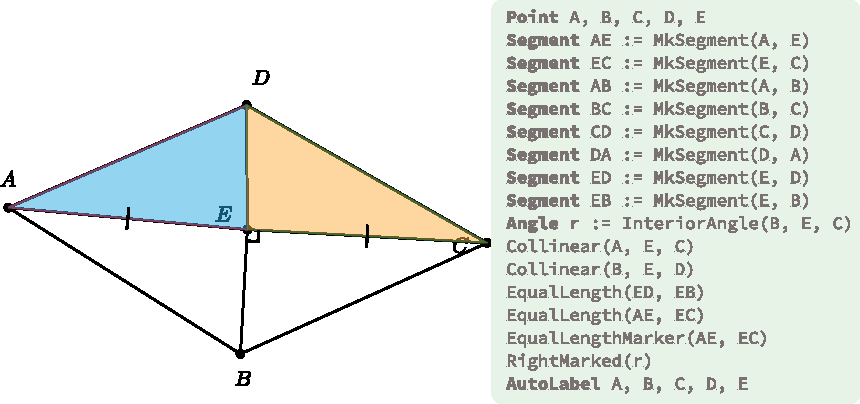
\includegraphics[width=\linewidth]{assets/congruence-example.pdf}
%     \end{center}
%     \caption{The example scenario of an Euclidean geometry problem.}
%     % \Description{This figure shows the diagram and Substance description of the example scenario in Figure 3. The diagram and Substance are identical to Figure 3.}
%     \label{fig:congruence-example}
% \end{figure}

% two-col
% \begin{figure}
%     \centering
%     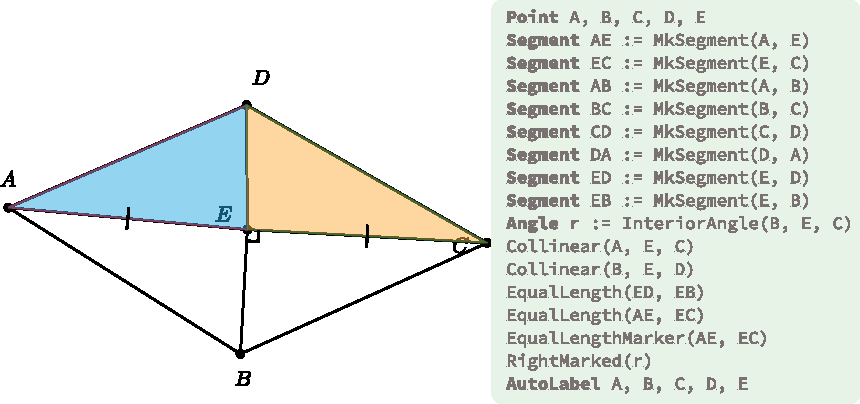
\includegraphics[width=\linewidth]{assets/congruence-example.pdf}
%     \caption{The example scenario of a Euclidean geometry problem.}
%     \Description{This figure shows the diagram and Substance description of the example scenario in Figure 3. The diagram and Substance are identical to Figure 3.}
%     \label{fig:congruence-example}
% \end{figure}

We use the problem in \cref{fig:edgeworth-problems} (left) to demonstrate how \Edgeworth generates variations that are meaningful as problem options. In the diagram shown, $\triangle DEC$ and $\triangle DEA$ are congruent by the Side-Angle-Side rule. In particular, they share a side ($DE$), the sides $AE$ and $EC$ appear to have equal length and are marked as such with a tick, and $\angle DEA$ and $\angle DEC$ are both right angles and therefore equal. 
% The diagram in \cref{fig:congruence-example} is replicated as Option 2 in \cref{fig:edgeworth-problems}. 
Option 4 in \cref{fig:edgeworth-problems} involves mutating the scenario by removing the right angle marker which makes it impossible to prove that $\angle DEA$ and $\angle DEC$ are equal. This is an example of the \textbf{Delete} mutation described in Section \ref{sec:edgeworth-mutation}. The angle appears to be a right angle in Option 3, so this option might serve as a good distractor for students still learning the distinction between the appearance of angles and their markings.

Option 3 involves mutating Option 2 by editing which sides have equal length. In Option 3, sides $CD$ and $AE$ are equal instead of $AE$ and $CE$. This is an example of the \textbf{Replace Arguments} mutation described in \cref{sec:edgeworth-mutation}. A student might incorrectly select Option 3 if they believed in a Side-Angle congruence rule, where a single angle and single side being equal could prove congruence. Finally, in Option 1 $\angle CEB$ neither is marked as a right angle nor appears as a right angle. A student might incorrectly select Option 1 if they believed in a Side-Side congruence rule, where two sides being equal could prove congruence.

\cref{fig:geometry-grid} shows the first 10 variations \Edgeworth generated from the example diagram. To create our problem, shown in \cref{fig:edgeworth-problems} (left), we selected the original diagram and two incorrect variations (numbers 1 and 8), plus another variation in an extended pool (number 16). As shown in \cref{fig:geometry-grid}, there are many other viable answer choices in the first 10 variations. Many of the diagrams involve extra details that are irrelevant to the problem, like the circle in number 6 or the vector above point B in number 2. These extra details can be pedagogically useful for teaching students to filter irrelevant information in the domain. Some of the other diagrams are very obviously incorrect, like number 10 which doesn't show a blue triangle, or number 7 where the blue triangle is much larger than the orange triangle; these can be useful for building confidence when students are first learning. 

% We assembled these problems from the diagrams alone. We did not look at the changes made to the textual scenario, and we do not expect our users to look at those textual changes. 

% \begin{figure}
%     \centering
%     \includegraphics[width=\linewidth]{assets/incorrect-mutants.pdf}
%     \caption{Three incorrect mutants (number 1, 8, and 16) selected for an Euclidean geometry problem (c04p01).}
%     \label{fig:incorrect-mutants}
% \end{figure}

% \cref{fig:incorrect-mutants} shows how \Edgeworth mutates the example scenario. For mutant 1, \Edgeworth changed \texttt{RightMarked(r)} to make $\angle BEC$ an obtuse angle, thereby violating the SAS rule. The resulting diagram is visually obvious because the colored triangles clearly have different shapes. Mutant 8 violates another predicate \texttt{EqualLength(AE, EC)} indirectly by changing the definition of $\overline{EC}$ to mean $\overline{CD}$. This is done by a combination of \textbf{Swap} and \textbf{Swap-In} mutations. The result is also a visually obvious incorrect diagram. Finally, mutant 18 changes \texttt{RightMarked(r)} to \texttt{RightUnmarked(r)} and also includes an irrelevant mutation that deletes $\overline{AD}$. Since the triangles are shaded, this extra mutation doesn't impact the readability of the resulting diagram. In fact, because $\angle BEC$ is still a right angle but not visually marked, it is a good distractor option for the problem. 




\subsection{General Chemistry: Lewis Structures}
\label{sec:chemistry}

% \begin{figure}[h]
%     \centering
%     \includegraphics[width=\linewidth]{assets/chemistry-problem.png}
%     \caption{An example problem in general chemistry that asks the student to identify the correct Lewis structure for HCN.}
%     \label{fig:chem-problem}
% \end{figure}

We chose 7 chemistry problems on Lewis structure from an online General Chemistry 1 course \cite{oli}. These problems test students' understanding of how atoms bond together based on formal charges. The module introduces students to the \textit{octet rule}: the tendency of main group atoms to form enough bonds to obtain eight valence electrons. Lewis structure diagrams show bonds among atoms and valence electrons on atoms typically following the octet rule. 

% To accurately assess student understanding and give them appropriate varied practice, it is important that problems (and solution options) in this module differentiate student understanding of these more particular principles:

% \begin{itemize}
%     \item The number of valence electrons in the outer shell is determined by the atomic number.
%     \item The most common molecular configuration minimizes free electrons. 
% \end{itemize}

We extend the existing \Penrose chemistry stylesheet to include notation and layout rules for Lewis structures. To permit incorrect diagrams, the chemistry stylesheet must not enforce the octet rule. It does specify that an atom can have any number of bonds and that it can have 0, 2, 4, or 6 valence electrons. These specifications cover all problem scenarios in this Lewis structure module.\footnote{``Odd electron molecules are very rare and cannot achieve full octets of electrons around atoms because of the odd number of electrons.'' \cite{oli}} In accordance with stylistic conventions in the field, \Edgeworth automatically lays out atoms, bonds, and electrons to maximize bond angles and repel electrons from bonds 
% (\eg \cref{fig:cocl2-example} and \cref{fig:edgeworth-problems} bottom-middle)
. For molecules involved in all 7 problems, the layout algorithm produces high-quality diagrams without any manual manipulation needed from the author. 

To configure \Edgeworth for this domain, we weight edits 100\%. We exclusively weight on edits because we observed that variations of molecules never add or delete atoms and bonds. Although valence electrons may be added or deleted, they are modeled as predicates that can be edited to change the number of electrons for an atom (\eg \sub{ZeroValenceElectrons(H)} $\rightarrow$ \sub{TwoValenceElectrons(H)}) via a \textbf{Replace Function} mutation operation. 

Figure~\ref{fig:edgeworth-problems} (middle) shows an \Edgeworth Lewis structure problem for hydrogen cyanide, with the correct diagram in the top-left. Incorrect choices for this problem can be generated via mutation. For instance, if a student forgets that nitrogen must have eight surrounding electrons, they might choose the bottom-left option, which was generated by removing the valence electrons around nitrogen. Or, if a student does not know that hydrogen should only have two electrons instead of eight, they might select the top-right choice, which was generated by mutating the number of electrons around hydrogen from zero to six. Finally, if a student does not know that free electrons should be minimized, they might pick the bottom-right diagram, which was generated by mutating up the number of electrons around carbon and nitrogen and changing the triple bond to a double bond.

\subsection{Discrete Math: Graphs}
\label{sec:graphs}

% \begin{figure}[h]
%     \centering
%     \includegraphics[width=\linewidth]{assets/graph-problem.png}
%     \caption{An example problem that asks the student to identify graphs with Euler circuits.}
%     \label{fig:chem-problem}
% \end{figure}

We draw 7 graph theory problems from the ``Graphs'' chapter of \textit{Discrete Mathematics and Its Applications} \cite[Chapter~10]{rosen1999discrete}.  We model our visual representation after the style used in the textbook, allowing students to recognize \Edgeworth-generated diagrams as they are already accustomed to recognizing graph diagrams. We created a new \Penrose stylesheet for four subdomains of graphs (directed vs not, and multigraph vs not). For each of these subdomains, \Edgeworth automatically lays out graph nodes, edges, loops, arrows, and labels in configurations that minimize confusing overlap of diagram elements. As with the other domains, no manual tweaking is necessary to obtain high-quality diagrams for problem variations. 
% The book defines six subdomains in Section 10.1, of which we use four:
% \begin{itemize}
%     \item \textit{Simple graph}---single undirected edges, no loops
%     \item \textit{Pseudograph}---multiple undirected edges, loops allowed
%     \item \textit{Simple directed graph}---single directed edges, no loops
%     \item \textit{Directed multigraph}---multiple directed edges, loops allowed
% \end{itemize}


To configure \Edgeworth for the graph domain, we weight additions 50\%, deletions 40\%, and edits 10\%. We disfavor edits in this domain because most of them are not useful: \textbf{Replace Function} is inapplicable for any of our graph subdomains, and \textbf{Swap Arguments} only applies to directed graphs. \textbf{Replace Arguments} is meaningful, but most desirable mutations for graphs are better represented by the addition or deletion of edges, or sometimes nodes. For instance, a bipartite graph can become not-so by adding edges, or a strongly-connected graph can become not-so by deleting edges. 

Figure~\ref{fig:edgeworth-problems} (right) shows an \Edgeworth problem asking which of four directed graphs have an Euler circuit. The bottom-right diagram does not have an Euler circuit, as can be seen by observing that the sum of $a$'s in-degree and out-degree is odd. In contrast, for the diagram in the bottom-left generated by deleting edge $(a, d)$, every node has an even sum of in-degree and out-degree, and indeed there does exist an Euler circuit. This condition on degree is only sufficient for undirected graphs, though; the diagram in the top-right is generated by flipping edge $(b, c)$ from the bottom-left diagram, but does not have an Euler circuit, thwarting the simple degree counting heuristic. Finally, the simple diagram in the top-left is generated by deleting $d$ and trivially has an Euler circuit. 



\section{Reliability Evaluation (\ref{rq:mut})}
\label{sec:reliability-eval}

\Edgeworth's approach involves random mutations. The mutation operations are type-safe, but type-safety does not prevent degenerate diagram layouts. For instance, \texttt{Point A, B; Triangle t := MkTriangle(A, A, B)} typechecks. However, since the triangle described in this scenario involves the \texttt{Point A} twice, \Edgeworth will produce a line segment, not a triangle from this scenario. Are \Edgeworth suggestions dominated by these nonsensical scenarios? In this section, we evaluate whether \Edgeworth can reliably suggest diagrams that are valid answer options to multiple-choice translation problems. 

\subsection{Methods}
\label{sec:reliability-method}

The goal of \Edgeworth is to generate enough diagram variations to assemble a four-choice multiple-choice problem for a given prompt. To this end, we use the following classification scheme for diagram variations: a variation can be a \textbf{Correct} or \textbf{Incorrect} answer to the prompt, or \textbf{Discard}ed because the diagram is invalid for missing key components or lacking readability.

For \ref{rq:mut}, we define ``relatively few variations'' to be 10 diagrams, and consider \Edgeworth to have generated a translation problem in $n$ variations if at that point we have (possibly including the original diagram) at least one \textbf{Correct} diagram, at least one \textbf{Incorrect} diagram, and in total at least four diagrams that are either \textbf{Correct} or \textbf{Incorrect}.

To evaluate this coding scheme, we randomly sampled 2 problems from each of our 3 domains, for 60 generated diagrams total. The first two authors each coded all 60 of those sample diagrams, after which we calculated the Cohen's $\kappa$ \cite{cohen1960coefficient} statistic. Then with the assumption that our coding scheme has reasonable inter-rater reliability, at least one author coded all remaining diagrams, allowing us to determine the number of our prompts for which \Edgeworth was able to successfully generate a multiple-choice problem. The coding results are included in supporting files.

\subsection{Results}

\subsubsection{Reliability of problem generation}

For \ref{rq:mut}, we found that \Edgeworth generated valid multiple-choice problems for 27/31 prompts within 10 variations, and for 30/31 problems within 20 variations. For each of these four failures with 10 variations, \Edgeworth did generate at least four \textbf{Correct} examples, but we had to \textbf{Discard} all the other diagrams, leaving no \textbf{Incorrect} examples. For the one remaining failure with 20 variations, \Edgeworth never succeeded even after we increased the number of variations to 50.


\subsubsection{Distribution}

\begin{table}
    \centering
    \begin{tabular}{r|rrr|r}
        & \textbf{Correct} & \textbf{Incorrect} & \textbf{Discard} & \textit{total} \\
        \hline
        geometry & 52 & 54 & 64 & 170 \\
        chemistry & 3 & 54 & 13 & 70 \\
        discrete & 28 & 25 & 17 & 70 \\
        \hline
        \textit{total} & 85 & 133 & 94 & 310
    \end{tabular}
    \caption{Distribution of diagram variation classes.}
    % \Description{This table describes the coding results from the reliability evaluation. There are four rows (blank, geometry, chemistry, discrete, and total) and five columns (blank, correct, incorrect, discard, and total). The first row and first column contain the headers. The numbers starting from row 2, column 2, in row order are: Row 2: 52, 54, 64, 170; Row 3: 3, 54, 13, 70; Row 4: 28, 25, 17, 70; Row 5: 85, 133, 94, 310}
    \label{tab:distribution}
\end{table}

The original diagram is a \textbf{Correct} answer for every prompt, except for the two Euler circuit prompts, in which the original diagram is \textbf{Incorrect}. For \Edgeworth-generated variations, the full distribution of classes is shown in Table~\ref{tab:distribution}.

The chemistry domain had a far smaller proportion of \textbf{Correct} variations than the other two domains because the only way for a variation to be \textbf{Correct} is for it to coincidentally be identical to the original diagram. Interestingly, in the other two domains, there were about the same number of \textbf{Correct} and \textbf{Incorrect} variations.

In the geometry domain, \textbf{Discard}ed diagrams were primarily either diagrams missing elements referred to in the question prompt, or diagrams that were visually degenerate (\eg everything compressed into a single line). In chemistry, we \textbf{Discard}ed diagrams where the molecule was disconnected. Finally, in the graph domain, we \textbf{Discard}ed diagrams in which some nodes were labeled and others were unlabeled (\ie \Edgeworth had inserted new unlabeled nodes when all nodes in the original diagram were labeled).

\subsubsection{Inter-rater Agreement}

We sampled two problems per domain from the problems collected in ~\cref{sec:edgeworth-case-studies} to evaluate inter-rater agreement (six problems total, 19\% of the dataset). We found perfect agreement on that sample, so $\kappa = 1$.


\section{Expert Walkthrough Demonstration and Feedback (\ref{rq:eco})}
\label{sec:expert-feedback}

The intended users of \Edgeworth are educators who create problems. These users are very important to the education system since other teachers make use of their problems. Therefore, we recruited educators who created visual practice problems in multiple domains and educational settings to evaluate ecological validity of \Edgeworth-generated problems (\ref{rq:eco}). While an expert survey may suffice for rating problem quality, we opted for walkthrough demonstration, based on prior research on evaluation methods by \citet{Ledo2018EvaluationResearch}, to gather additional qualitative feedback on the value of having the toolkit in their day-to-day work.

\subsection{Participants and Procedure}
\label{sec:expert-procedure}

We recruited domain expert educators of chemistry, geometry, and graph theory. Experts were invited based on their extensive teaching experience in the domain and past experience in \emph{authoring} diagrammatic content. In contrast to the criteria in the formative study (\cref{sec:edgeworth-formative}), this study selected participants based on their domain-specific expertise in authoring problems. Recruited educators came from a wide range of institutions, including MOOC platforms, liberal arts colleges, community colleges, research universities, and secondary schools. The average teaching experience among the 9 expert educators (E1–E9) was 10.33 years, with a standard deviation of 8.39 years, highlighting a broad range of teaching experience. One of the participants is the author of problems in one of the domains in \cref{sec:edgeworth-case-studies}.
\cref{tab:demographics} summarizes the demographic information for 9 expert educators (E1--9) who participated in the study. 

\begin{table}
    \centering
    \begin{tabular}{l|l|l}
        \textbf{Occupation} & \textbf{Yrs} & \textbf{Domain(s)}    \\
        \hline
        MOOC Course Designer       &  7 & Chemistry           \\ 
        Liberal Arts College Prof. &  4 & Chemistry, Geometry \\
        Community College Prof.    & 30 & Chemistry           \\
        Liberal Arts College Prof. & 11 & Graphs              \\
        Research University Prof.  & 17 & Graphs              \\
        Research University Prof.  &  5 & Graphs              \\
        Middle School Teacher      &  5 & Geometry            \\
        Undergraduate TA           &  3 & Geometry, Graphs    \\
        High School Teacher        & 11 & Geometry, Graphs    \\
    \end{tabular}
    \caption{Participant demographics in walkthrough demonstration sessions.}
    % \Description{A table showing the demographics of participants in walkthrough demonstration sessions. It has four columns labeled: ID, Occupation, Teaching Experience, and Domain(s). The entries are: E1 as a MOOC Course Designer with 7 years in Chemistry, E2 as a Professor at a Liberal Arts College with 4 years in Chemistry and Geometry, E3 as a Professor at a Community College with 30 years in Chemistry, E4 as a Professor at a Liberal Arts College with 11 years in Graphs, E5 as a Professor at a Research University with 17 years in Graphs, E6 as a Professor at a Research University with 5 years in Graphs, E7 as a Middle School Teacher with 5 years in Geometry, and E8 as an Elementary School Tutor and Undergraduate TA with 3 years in Geometry and Graphs.}
    \label{tab:demographics}
\end{table}

Each expert participated in a 60- to 90-minute session via video conferencing, which was recorded with their consent. At the start of each session, we demonstrated the workflow of \Edgeworth end-to-end, as described in \cref{sec:edgeworth-workflow}, on one problem outside of the expert's domain. For the remainder of the session, we asked the expert to evaluate two to four problems sampled from \cref{sec:edgeworth-case-studies} in their domain. Per problem, the expert rated 10 diagram variations based on the categories described in \cref{sec:reliability-method}. In addition, we asked participants to provide more granular feedback on diagram quality. After rating the diagram variations, they were asked to pick diagrams to assemble a four-choice diagrammatic translation problem. After the problem was assembled and shown on the interface, we asked (1) if they would use the problem in their instruction and (2) how they would author the diagram using their own workflow. The full study protocol is included in supporting files.

% \subsection{Existing Problem Authoring and Diagramming Processes}

% % thesis: diagramming is a design problem and experts 

% % use of diagrams
% Experts report a wide range of diagram use such as problem sets (E1, E3, E4, \hl{E9}), worked examples (E2--\hl{9}), tests (E1, E2), and in-class activities (E2, E7). Most experts favor multiple-choice translation problems, especially when \quotei{the class size grows} (E2). A few experts favor free-response questions for better feedback to students but noted the scalability problem with them (E2, E3, E7, \hl{E9}). For instance, E3 pointed out that they \quotei{can't monitor how 75 students are drawing a Lewis structure.} 

% % diagram is hard
% To make diagrams, experts used tools such as Microsoft Powerpoint (E1, E3), LaTeX (E4, E5, E6, E8), InkScape~\cite{bah2011inkscape} (E4), Geogebra~\cite{geogebra5} (E2, E7), \hl{and Desmos}~\cite{desmos} (E9). Similar to prior studies on diagramming tools~\cite{naturalDiagramming}, they reported barriers to using these tools that led to \quotei{painful} (E1, E2, E5, E6, E8) diagramming processes. As a result, if possible, they often fell back to hand-drawn diagrams because they \quotei{take less time} (E1, E4, E6), but E5 noted drawing skill is \quotei{one of the talents I did not have and I wish I did.} High-quality diagrams also take significant crafting to get right. For example, E4 would still \quotei{easily spend a day} on a figure because \quotei{if I start trying to make a perfect vector graphics version of it, it's inevitable. We just go down a rabbit hole of trying to make it look nicer and nicer.} 

\subsection{Ecological Validity of Generated Problems (\ref{rq:eco})}

Overall, experts were happy with the problems they assembled with \Edgeworth-generated diagrams. Experts (E1--9) indicated that they would use all of the problems they created using \Edgeworth in their coursework. Other experts said they would use \Edgeworth-generated problems \quotei{early in the learning process} (E3) and \quotei{as a warm up exercise at the start of the next lecture} (E4). In addition, the problems can be used to review previously introduced concepts. For example, E3 found the diagram variations that break the octet rule to be useful for \quotei{after you've also introduced expanded octet or non-octet-rule things.} Experts plan to use \Edgeworth-generated problem to \quotei{focus on things that students struggle with} (E3) and when introducing concepts that are \quotei{all about visualization} (E5) such as planarity of graphs. E7 was excited to use problems we created in the expressiveness evaluation (\cref{sec:edgeworth-case-studies}) in their class because they were \quotei{going to be covering everything [on the list].} In addition to just asking students to select correct diagrams, E3 also pointed out that by prompting students to \quotei{tell me what is wrong rather than just which is the correct one,} the problem can be used to \quotei{dive deeper.} Similarly, E4 proposed to use \Edgeworth problems as \quotei{an interactive warm-up for reviewing the last lecture, where students vote on and explain why a diagram is correct.} E7 even plans to use \Edgeworth as \quotei{a creative instead of assessment piece} and \quotei{have the students be the teacher \dots{} playing this role more, they get better at tests, because they understand what the test makers are doing.} 

\subsection{Expert Feedback}

% \subsubsection{Experts provided positive qualitative feedback on \Edgeworth}
% fast and good
Experts reacted positively to \Edgeworth. They found \Edgeworth to be a \quotei{perfect fit} (E1, E6, E8) for generating multiple-choice problems, especially \quotei{low-stake} (E2, E3, E5, E6, E8, \hl{E9}) quizzes that \quotei{incentivize [students] to keep up with the class} (E8). Experts said the automatic layout of \Edgeworth \quotei{draws things really fast} (E5), \quotei{saves you the time of drawing multiple structures} (E3), and produces \quotei{beautiful} (E4, E7) diagrams. Comparing with their existing tools, \Edgeworth is a \quotei{nice time-saver} (E3) and the translation problems they authored during the session would take an \quotei{enormous amount of work} (E4), \quotei{infinitely longer than this took} (E6).

Notably, experts pointed out that \Edgeworth aids creativity by promoting \quotei{recognition over recall} (E6). Specifically, \Edgeworth helps with \quotei{the thinking about how to come up with the graphs} and simplifies the diagram layout such that \quotei{you just generate some mutations that you click refresh until it looks nice} (E6). E2 liked that \quotei{it can come up with different possibilities than the ones that would be immediately apparent to me.} 

In addition, experts commented that \Edgeworth can enable them to give students more practice. For instance, E4 noted that \quotei{there's a feedback loop where \dots{} if I had a really good tool for generating nice multi-choice questions, then I could envision doing that much more frequently.}  

% Importantly, in the context of student authoring problems themselves, E7 thinks that lowering the barrier of problem authoring help students \quotei{feel they have ownership in their learning as well as sharing their ownership with other students in the class.}

% \subsubsection{Experts used visual selection to express diverse standards on diagram quality}

% When rating diagram mutants, experts agreed with diagram ratings of \cref{sec:reliability-eval}, but expressed unique standards for selecting answer choices (\cref{sec:expert-procedure}). Since experts had different standards, they selected different diagrams to assemble problems. This suggests \Edgeworth's use of visual selection met experts' needs.

% One group of experts (E2, E4, E6, E7, E8, \hl{E9}) preferred to maintain a balanced mix of answer choices, \quotei{at least one that's obviously correct, at least one that's obviously incorrect, and then \dots{} two where you have to think about that a little bit} (E6). One rationale was to \quotei{make sure [the problem] is challenging enough, but also has some things that are accessible to students that haven't completely mastered the material} (E4). Another was to teach \quotei{the process of elimination} (E7, \hl{E9}). Another group of experts (E1, E3, E5) had much higher standards for including a mutant in a multiple-choice problem. For example, E1 preferred problems to contain one correct answer and multiple distractor options that are \quotei{less obvious} such that students won't \quotei{pattern match without looking at the details.}

% % On a problem that E2 accepted 7 out of 10 mutants as good incorrect options, E3 discarded 8 out of 10 because they \quotei{violated the octet rule in egregious or blatantly egregious way.} However, E3 said whether the octet rule can be broken depends on \quotei{where students are in the course.}

% The difference of standards is highly individual. From E2's knowledge of \quotei{colleagues [who] only give difficult distractors} and \quotei{certain profs [who] are legendary for having really hard multiple choice,} they guessed that harder problems \quotei{motivate the students to try harder,} but also pointed out that it \quotei{only works for certain students in my experience.} E3 stated that their choice in diagrams \quotei{hinges upon my perception of whether students will automatically disqualify something,} which they admitted is \quotei{a certain premise or bias.}  In E3's words: \quotei{Wow, it's really tough to \dots{} completely take off the instructor hat.} 

% This comment reflects the concept of \textit{expert blind spot} in learning sciences literature, where experts fail to \quotei{understand the processes of novices who are struggling to understand new ideas during their constructive learning process} ~\cite{expertBlindspot}.

% \subsubsection{Experts selected isomorphic diagrams to build conceptual understanding}

\Edgeworth sometimes produces isomorphic diagrams, \ie diagrams with identical content but different layouts. These diagrams occur when \Edgeworth's mutations have no net impact on the example diagram, \eg the mutator removes an edge from a graph and adds it back. Surprisingly, experts found value in these isomorphic diagrams. 
In their geometry course, E2 said that their textbook's diagrams \quotei{get drawn the same way over and over again. And some students get stuck into thinking that the concept is only communicated when the diagram is drawn [exactly] that way.} When assembling a problem about the $HCN$ molecule, E3 compared two isomorphic variations, and picked one over another because \quotei{it's drawn the opposite \dots which is interesting and I think students are going to get it wrong.}  Similarly, E1 finds isomorphic diagrams to be useful for \quotei{molecules with resonance structures.} 
% However, for simpler molecules, E1 cautioned that might mislead students to think that \quotei{they are different structures when they really are the same.} 
E5 found isomorphic planar graphs to be particularly useful because students find them \quotei{painstaking to visualize when they just started.} E5 planned to use \Edgeworth to \quotei{draw a graph that doesn't look like it could be planar first, but then untangle it to show that the graph is actually planar.}


\section{Definitions}
\label{sec:definitions}

In the discussion of translation problems, \cref{chp:edgeworth} uses terms such as ``instance,'' ``noninstance,'' ``near hit,'' and ``near miss.'' To standardize the terminologies in this appendix, I give some definitions here.

Given a set of mathematical statements describing logical entities and their relationships, a diagram can be associated with them in one of the following ways:

\vspace{0.5em}
\begin{figure}[h]
\begin{minipage}[b]{0.48\linewidth}
$\bullet$ \textbf{Example}: the diagram represents the math statements, \ie all the statements hold true in the diagram. 
    \vspace{3pt}
    
$\bullet$ \textbf{Counterexample}: the diagram clearly violates the math statements, \ie one or more statements are false in the diagram.
    \vspace{3pt}
    
$\bullet$ \textbf{Positive edge case}: the diagram is an example of the math statements, but contains extraneous entities and/or more specialized relationships. 
    \vspace{3pt}
    
$\bullet$ \textbf{Negative edge case}: the diagram is a counterexample, but only requires a few changes to become an example.
\end{minipage}
\hfill
\begin{minipage}[b]{0.45\linewidth}
    \centering
    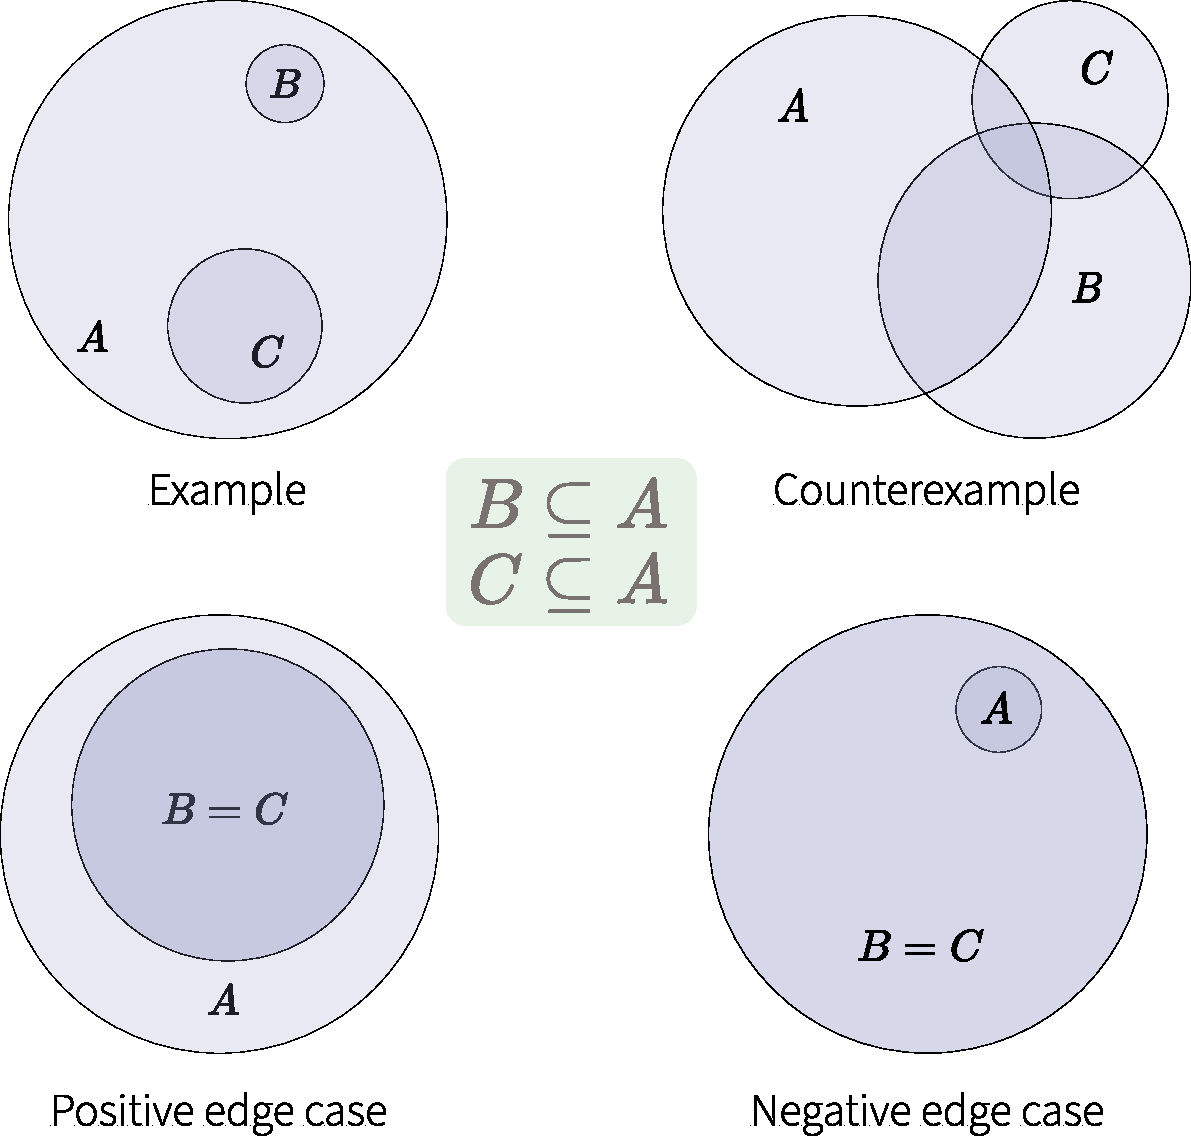
\includegraphics[width=\textwidth]{assets/appendix/definitions-examples.pdf}
\end{minipage}
\end{figure}

% While distinguishing between examples and counterexamples is often straightforward, identifying edge cases can depend on the context. For instance, the counterexamples in the figure above both violate all math statements, but the lower-right diagram can be considered an edge case because one can swap the labels $A$ and $B$ to make it an example. 

\section{Summary of proposed work}

\subsection{Programming-by-example workflow}


\begin{figure}
    \centering
    \includegraphics[width=\linewidth]{assets/appendix/edgeworth-bad-output.pdf}
    \caption{A screenshot of the \Edgeworth interface, after generating examples for a translation problem focusing on improper subsets. Because of the configuration, pool of mutant diagrams aren't suitable for this problem.}
    \label{fig:edgeworth-bad-output}
\end{figure}


With the \Edgeworth mutator, the primary mode of interaction is configuration-based: the author creates a mutator configuration and the mutator generates a set of diagrams. When these diagrams don't satisfy the needs of the author (\eg missing counterexamples that are important for an educational goal), the author can only edit the configuration again and hope to get better ones. In short, the quality of \Edgeworth-generated diagrams are sensitive to the configuration. 

For example, suppose an author would like to create translation problems that test students' knowledge of improper subsets, especially the fact that if $A \subseteq B$, $A = B$ is allowed. Using the \Edgeworth mutator, the author first creates a prompt \Substance program:

\begin{verbatim}
Set A, B, C
IsSubSet(B, A)
IsSubset(C, A)
\end{verbatim}

Not familiar with how program mutator works, the author picks a few options in the configuration interface and clicks ``Generate Diagrams.'' Ideally, \Edgeworth should generate a set of examples of the subset relations that include the edge cases of $A = B$, $A = C$, or $B = C$, and counterexamples of $B \not\subseteq A$ or $C \not\subseteq A$. 

However, the output from \Edgeworth seems too random (\cref{fig:edgeworth-bad-output}). There are useful counterexamples, but none of the diagrams include edge cases such as:
\begin{verbatim}
Set A, B, C
IsSubSet(B, A)
IsSubset(C, A)
Equal(B, C)
\end{verbatim}

In other words, without intimate knowledge of how the \Edgeworth mutator is configured, the author cannot express their intent easily. In this case, it's much more natural to write a few examples from scratch, or manually make slight tweaks to examples in the mutant pool. I propose to \textbf{create a programming-by-example (PBE) workflow, where the author manually creates or edits a few diagrams, and \Edgeworth generates more diagrams with similar properties.}

Using this workflow for the example above, the author can manually create a few examples by directly editing the prompt program. In this case, the author adds the \sub{Equal(B, C)} predicate. Their intent is to include the edge case of improper subsets in this problem, where some of the subset relations are actually equality. \Edgeworth generates a set of similar examples that add \sub{Equal} predicates with existing identifiers in different ways. 

\vspace{10pt}
\begin{figure}[h]
    \centering
    \includegraphics[width=0.8\linewidth]{assets/appendix/synthesis-driven-workflow.pdf}
    % \caption{Caption}
    % \label{fig:my_label}
\end{figure}
\vspace{10pt}

The addition of \sub{Equal(B, C)} is effectively a user-generated mutation, and \Edgeworth needs to understand this mutation to generate similar instances. To do so, the \Edgeworth synthesizer matches a series of author edits to predefined mutations. Once the synthesizer finds a mutation path that describes the author edit, it can then inform the mutator to generate examples with similar properties (\ie including the edge case of equal sets). Using this workflow, the author can rapidly author diagrams that belong to a particular category in the translation problem. For example, the problem below has diagrams that include set equalities as correct answers, and diagrams that violate one or both subset relations as incorrect answers.

\vspace{10pt}
\begin{figure}[h]
    \centering
    \includegraphics[width=0.8\linewidth]{assets/appendix/translation-problem-sets.pdf}
    % \caption{Caption}
    % \label{fig:my_label}
\end{figure}
\vspace{10pt}

\subsection{Automatic detection of examples and counterexamples}
\label{sec:autodetect}

One key application of \Edgeworth is generating translation problems with examples and counterexamples. Therefore, it's important for the system to understand whether a diagram is an example or counterexample of the prompt. However, the \Edgeworth mutator performs \Substance program mutations on the prompt without knowing if a mutant is semantically equivalent to the prompt. To address this, I propose to \textbf{automatically detect examples and counterexamples}.

One heuristic is cross-instance energy evaluation (CIEE) described in~\cref{sec:mutation}.  CIEE determines the distance between two \Substance programs by examining visual constraint satisfaction. 

Another approach is to provide the \Edgeworth mutator with more semantic information such that it generates examples and counterexamples by construction. Currently, none of the mutation operators carry any mathematical semantics because \Domain doesn't contain enough information. For instance, many mathematical predicates have reflexive, symmetric, transitive, and substitution properties, but \Domain only encodes basic type definitions. For a more precise notion of correctness, I plan to extend \Domain to model such properties, and use them in the \Edgeworth mutator, possibly together with CIEE, to generate higher quality mutants.  

\subsection{Hypotheses and research questions}

Comparing with related work discussed in \cref{sec:edgeworth-related}, \Edgeworth uniquely support scalable generation of diagrammatic translation problems in multiple domains. Therefore, in this section, I discuss hypotheses that cover the essential features of \Edgeworth such as the mutation-based approach and automatic detection of examples and counterexamples. For each hypothesis, I will also discuss further research questions to be investigated in the evaluation plan. 

\boxtext{\textbf{H1:} Given manageable effort in configuring the mutator, \Edgeworth can reliably generate examples and counterexamples for translation problems with relatively few mutants required.}

An effective translation problem needs to include both examples and counterexamples. Therefore, the technical approach of \Edgeworth---program mutations on \Substance code---must produce them reliably. To verify H1, the following research questions need to be answered:

\begin{itemize}
    \item \textbf{R1.1}: How many mutants does \Edgeworth need to generate to obtain sufficient examples and counterexamples for translation problems?
    \item \textbf{R1.2}: How frequently does \Edgeworth succeed or fail at doing so?
\end{itemize}

The preliminary evaluation showed that the mutator configuration will affect the quality of the mutants. Therefore, I will also address the following research question on mutator configuration and will use the results to further investigate possible ways to lower the configuration burden, e.g. the programming-by-example workflow and changes to the configuration format.

\begin{itemize}
    \item \textbf{R1.3}: How much configuration effort is required to produce examples and counterexamples? 
\end{itemize}

\boxtext{\textbf{H2}: \Edgeworth makes translation problem authoring more efficient.}

The main goal of \Edgeworth is to improve the efficiency of translation problem authoring. To verify H2, the evaluation plan will answer:
\begin{itemize}
    \item  \textbf{R2.1}: Comparing with workflows that authors are using, can \Edgeworth shorten the authoring time of translation problems?
    \item  \textbf{R2.2}: Which aspect(s) of the authoring workflow does \Edgeworth simplify, and does \Edgeworth introduce new authoring difficulties? 
    \item  \textbf{R2.3}: Are authors more efficient using the configuration-based workflow or programming-by-example workflow?
\end{itemize}

Regardless of the answer to R2.1, meaningful results on R2.2 can provide more insights on how \Edgeworth's approach impacts the problem authoring experience. For instance, I postulate that \Edgeworth improves authoring efficiency by (1) simplifying the mechanics of diagram production and (2) reducing the author's effort to come up with examples and counterexamples. On the other hand, \Edgeworth's mutation-based approach may introduce new problems such as difficulties finding the right diagrams from the mutant pool and controlling the quality of examples. The automatic detection heuristics described above aim to mitigate these difficulties.

\boxtext{\textbf{H3}: \Edgeworth can automatically distinguish examples from counterexamples, and this feature helps authors find examples and counterexamples for translation problems.}

The effectiveness of translation problems depends on the choice of examples and counterexamples. I hypothesize that example generation/selection is a nontrivial activity that authors spend time doing, and computational support in \Edgeworth can help authors identify examples/counterexamples. Answering the following research questions will verify H3:

\begin{itemize}
    \item \textbf{R3.1}: Can \Edgeworth automatically detect examples, counterexamples, and edge cases with a reasonably high accuracy?
    \item \textbf{R3.2}: Do the detection results help authors identify potential answers to translation problems?
\end{itemize}


\section{Plan}

\subsection{Pilot usability evaluation}

To prepare the \Edgeworth prototype for evaluation, I will first evaluate the usability of \Edgeworth by recruiting authors to perform small authoring tasks with the \Edgeworth prototype. For example, the participants may be asked to author a simple diagrammatic translation problem. The goal of this pilot study is to identify missing features, usability problems, and opportunities for simplification. The study may include several rounds with increasingly high-fidelity prototypes. After each round, I will refine the design and implement the next prototype. Here are some possible high-level questions for the study:
\begin{itemize}
    \item What are the key design considerations for translation problem authoring? How do they fit with the features of \Edgeworth?
    \item How do authors prefer to work with \Edgeworth? When do they opt to write a configuration file and generate many diagrams? When do they use the by-example workflow? Do they mix the two workflows?
    \item How does the experience compare to their existing tools? How can \Edgeworth incorporate useful parts of them? 
\end{itemize}

\subsection{Technical evaluation of automated production of diagram problems}
\label{sec:case-study}

While the preliminary study (\cref{sec:edgeworth-prelim-eval}) shows some promise of \Edgeworth's approach, the data from this study is insufficient for investigating H1 and R1.1-3. In this study, I will investigate if \Edgeworth can reliably produce diagrams for translation problems (H1) by gathering richer data on its success rate, efficiency, and human effort. 

\subsubsection{Translation problem set} 

I will reproduce diagrammatic problems from the same geometry textbook~\cite{holtGeometry} used in \cref{sec:edgeworth-prelim-eval}. In the textbook, diagrammatic problems often require representational fluency but aren't presented as multiple-choice translation problems with diagrams as choices. I plan to start with the original set of 24 translation problems that were reframed from textbook problems, and potentially extend the dataset using the same methodology of reframing the problems. Each translation problem in the dataset will include (1) a textual prompt, (2) four diagrams, and (3) a \Substance prompt program.

\subsubsection{Data collection} 

The output of \Edgeworth may be sensitive to factors like randomness of mutation paths and quality of configuration. Therefore, for each of the translation problems in the dataset, I will use the configuration-based workflow (\cref{sec:mutation}) in \Edgeworth to produce multiple problem instances. Each valid problem instance is a multiple-choice translation problem with four diagrams comprised of examples, counterexamples, and edge cases of the problem prompt. The validity of problem instances is determined manually during the study. 

Each problem instance may take multiple trials of executing the mutator and editing the configuration. The authoring process for each problem instance will be screen-recorded and documented. \Edgeworth will also be instrumented to log data such as the following:

\begin{itemize}
    \item Mutator data: mutant diagrams and their mutation paths, number of mutant generated per trial.
    \item Execution history: configuration file per execution and mutants selected for the translation problem.
    \item Edit history of the configuration: edits to a configuration for a particular translation problem and changes to configuration schema between translation problems.
\end{itemize}

\subsubsection{Proposed methodology} 

For R1.1, I plan to count (1) the number of mutants generated over multiple trials to obtain a valid problem instance and (2) the number of mutants in the last successful trial. The average of (2) over all translation problems measures the reliability of \Edgeworth given a good configuration, whereas that of (1) factors in the human effort of authoring such a configuration. To answer R1.2, I will run \Edgeworth with the configuration of the last successful trial, and measure the success rate of producing valid problem instances. 

For R1.3, I will use the screen recording to measure the time-to-completion for each valid problem instance and also count trials-to-completion. These data may be subject to particular contexts in which I will run the study. To gain a more objective understanding of the complexity of configuration files, I will also measure the specificity of the configuration to help answer R1.3. As a base case, an empty configuration with defaults takes no human effort to author, and a configuration that selects many constructs from \Domain takes significantly more effort. I will use the edit history and the length of the resulting configuration file itself to measure configuration effort.

% As discussed in \cref{sec:definitions}, while it's straightforward to distinguish between examples and counterexamples
The validity of edge cases depends on the context of a particular translation problem.  For all of the problems, I will label examples, counterexamples, and edge cases, and document the context and my rationale.  In addition, I will recruit a geometry teacher to label a sample of the problems from the dataset. I will then calculate the inter-rater reliability of between my rating and the teacher rating to assess whether my rating agrees with expert judgments. 

Then, I will use \Edgeworth to perform automatic detection (\cref{sec:autodetect}) on all translation problems from this study, and compute inter-rater reliability between the manual labels and detection results. Along with the documented edge case decisions from the study, a high inter-rater reliability can provide more confidence that \Edgeworth can accurately detect positive and negative edge cases (R3.1). 

\subsection{Experimental evaluation of authoring efficiency}

This study is an authoring experiment that compares (1) \Edgeworth against existing authoring tools and (2) features of \Edgeworth (\eg configuration vs. PBD, auto-detection on/off). Participants will create diagrammatic translation problems using conventional drawing tools or \Edgeworth. For H2, this study quantitatively measures the efficiency with or without \Edgeworth, compare between configuration-based and PBD workflows, and gather qualitative data on how \Edgeworth improves and/or hinders translation problem authoring. For H3, this study will test within-subjects whether the automatic detection feature helps participants in distinguishing and generating examples and counterexamples. 

\subsubsection{Tasks}

All participants will be asked to complete 4 translation problem authoring tasks, each sampled from the case study dataset (see \cref{sec:case-study}). For each task, the participant will be given (1) an textual problem prompt and (2) an example diagram (\ie a correct response to the prompt). Participants will create 3 instances of this problem, each with two examples and counterexamples (12 diagrams in total). In the participant is using \Edgeworth, they will also be given (3) a \Penrose trio corresponding to the prompt. 

\subsubsection{Proposed methodology}

The participants will be divided into 3 groups, each group distinguished by the tool being used: 
\begin{itemize}
    \item Control group: a conventional drawing tool\footnote{During recruitment, we will survey the participants to find a common tool they know}, \eg Google Drawings
    \item \Edgeworth-config group: \Edgeworth with the configuration-based interface
    \item \Edgeworth-PBD group: \Edgeworth with the PBD interface
\end{itemize}
For both \Edgeworth groups, the automatic detection feature will be enabled for 50\% of the tasks. Below is an example of the study setup, where D indicates \Edgeworth with automatic detection and N without.

\begin{table}[h]
\centering
\begin{tabular}{l|cccccc}
                    & Task 1 & Task 2 & Task 3 & Task 4  \\ \hline
Control             &   -    &    -   &    -   &   -   \\ 
\Edgeworth-config 1 & N      & D      & D      & N   \\
\Edgeworth-config 2 & D      & N      & D      & N   \\
\Edgeworth-PBD 1    & D      & N      & N      & D   \\
\Edgeworth-PBD 2    & N      & D      & N      & D   \\
\end{tabular}
\end{table}
Between tasks, participants will be asked to explain how they came up with examples and counterexamples, identified useful edge cases, and interacted with the authoring tool. The study sessions will be recorded and transcribed. 

The recording and \Edgeworth data will be analyzed to measure the authoring time for each task. The total authoring time difference between the conventional drawing tool and \Edgeworth will be used to answer R2.1. The time difference between \Edgeworth-config and \Edgeworth-PBD will answer R2.3. I will also observe the relative time participants spend on writing configuration in \Edgeworth-config and \Substance code in \Edgeworth-PBD. This observation will provide an estimate of the overhead of each workflow. Finally, I will compare the time with or without automatic detection (R3.2). 

If participants do spend less time with automatic detection enabled, there may be two possible sources of this speedup: (1) they can filter down mutant diagrams in \Edgeworth more quickly, \ie less tool interaction; (2) \Edgeworth helps offload the effort in identifying examples and counterexamples, \ie less example ideation. Participants' answers between tasks will help us determine which of these reasons is dominant (R2.2).

The video recordings will be coded to identify challenges participants encounter in both the conventional drawing tool and configuration-based or PBD \Edgeworth (R2.2, R2.3), and how they interact with the automatic detection result (R3.2). 

\section{Milestones and timeline}

\cref{fig:timeline} shows a plan for the sequence of the proposed work mapped to a timeline.

\vspace{10pt}
\begin{figure}[h]
\begin{center}
\begin{ganttchart}[y unit title=0.4cm,
y unit chart=0.5cm,
x unit=0.32cm,
vgrid,hgrid, 
title label anchor/.style={below=-1.6ex},
title left shift=.05,
title right shift=-.05,
title height=1,
progress label text={},
bar height=0.7,
group right shift=0,
group top shift=.6,
group height=.3]{1}{40}
%labels
\gantttitle{Fall 22}{11} 
\gantttitle{Spring 23}{11} 
\gantttitle{Summer 23}{7} 
\gantttitle{Fall 23}{11} 
\\
%tasks
\ganttbar{Usability Pilot}{1}{1} \\
\ganttgroup{System Impl.}{1}{16} \\
\ganttbar{Config system}{1}{4} \\
\ganttbar{PBD system}{9}{16} \\
\ganttgroup{Technical eval.}{3}{12} \\
\ganttbar{Dataset}{3}{4} \\
\ganttbar{Experiment}{5}{8} \\
\ganttbar{Analysis}{9}{10} \\
\ganttbar{Writeup}{11}{12} \\
\ganttgroup{Experimental eval.}{12}{28} \\
\ganttbar{Authoring Pilot}{15}{16} \\
\ganttbar{IRB \& Design}{12}{16} \\
\ganttbar{Recruitment}{14}{16} \\
\ganttbar{Experiment}{17}{23} \\
\ganttbar{Analysis}{24}{25} \\
\ganttbar{Writeup}{26}{28} \\
\ganttgroup{Dissertation}{29}{40} \\
\ganttbar{Drafting}{29}{36} \\
\ganttmilestone{Defense}{40}
% \ganttbar{task 3}{9}{10} \\
% \ganttbar{task 4}{11}{15} \\
% \ganttbar[progress=33]{task 5}{20}{22} \\
% \ganttbar{task 6}{18}{19} \\
% \ganttbar{task 7}{16}{18} \\
% \ganttbar[progress=0]{task 8}{21}{24}

% %relations 
% \ganttlink{elem1}{elem2} 
% \ganttlink{elem3}{elem4} 
% \ganttlink{elem1}{elem5} 
% \ganttlink{elem3}{elem5} 
% \ganttlink{elem2}{elem6} 
% \ganttlink{elem3}{elem6} 
% \ganttlink{elem5}{elem7} 
\end{ganttchart}
\end{center}
\caption{Timeline of \Edgeworth projects}
\label{fig:timeline}
\end{figure}